%%%%%%%%%%%%%%%%%%%%%%
\documentclass{doublecol-new}
%%%%%%%%%%%%%%%%%%%%%%
\usepackage{natbib,stfloats}
\usepackage{mathrsfs}
\usepackage{epstopdf}
\usepackage{graphicx}


\def\newblock{\hskip .11em plus .33em minus .07em}

\theoremstyle{TH}{
\newtheorem{lemma}{Lemma}
\newtheorem{theorem}[lemma]{Theorem}
\newtheorem{corrolary}[lemma]{Corrolary}
\newtheorem{conjecture}[lemma]{Conjecture}
\newtheorem{proposition}[lemma]{Proposition}
\newtheorem{claim}[lemma]{Claim}
\newtheorem{stheorem}[lemma]{Wrong Theorem}
\newtheorem{algorithm}{Algorithm}
}

\theoremstyle{THrm}{
\newtheorem{definition}{Definition}[section]
\newtheorem{question}{Question}[section]
\newtheorem{remark}{Remark}
\newtheorem{scheme}{Scheme}
}

\theoremstyle{THhit}{
\newtheorem{case}{Case}[section]
}

\makeatletter
\def\theequation{\arabic{equation}}

%\JOURNALNAME{\TEN{\it Int. J. System Control and Information
%Processing,
%Vol. \theVOL, No. \theISSUE, \thePUBYEAR\hfill\thepage}}%
%
%\def\BottomCatch{%
%\vskip -10pt
%\thispagestyle{empty}%
%\begin{table}[b]%
%\NINE\begin{tabular*}{\textwidth}{@{\extracolsep{\fill}}lcr@{}}%
%\\[-12pt]
%Copyright \copyright\ 2012 Inderscience Enterprises Ltd. & &%
%\end{tabular*}%
%\vskip -30pt%
%%%\vskip -35pt%
%\end{table}%
%}
\makeatother

%%%%%%%%%%%%%%%%%
\begin{document}%
%%%%%%%%%%%%%%%%%

\setcounter{page}{1}

\LRH{Deep Learning in Information Retrieval}

\RRH{Deep Learning in Information Retrieval}

%\VOL{x}

%\ISSUE{x}

%\PUBYEAR{xxxx}

\BottomCatch

%\CLline

\PUBYEAR{2018}

\subtitle{}

\title{Deep Learning in Information Retrieval}

%
\authorA{Saba Kanwal(18L-1860)}
%
\affA{Department of Computer Science,\\ Fast University,\\ Lahore, Pakistan \\
Fax: +1 \qquad E-mail: l181860@lhr.nu.edu.pk}
%
%
\authorB{Maham(18L-1886)}
\affB{Department of Computer Science,\\ Fast University,\\ Lahore,Pakistan \\
Fax: +1 \qquad E-mail: l181886@lhr.nu.edu.pk}
%

%
%\authorA{Fusheng Wang\footnote{Work done while working at Siemens Corporate Research.} }
%
%\affA{Department of Biomedical Informatics, Emory University
%\newline
%36 Eagle Row, Ste 589, Atlanta, GA 30322, USA}
%
%
%
%\authorB{\footnotesize Cristobal Vergara-Niedermayr\footnote{Work done while working at Siemens Corporate Research.}}
%\affB{Oracle \newline
 %New Jersey, USA}
%
%


\begin{abstract}
Deep learning is one of powerful tool that is used to represent complex internal representations with the help of neural network. In information retrieval, deep learning comes into action in case of hard problems. Hard problems in IR are matching of image with text, generating of answers based on some given facts, answer question based on facts in knowledge base and many other problems discussed in detail in this paper. Deep learning basic units in IR are RNN, CNN, word embeddings, and neural networks.The fundamental problem areas in IR that needs deep learning solutions are to learn distributed representation of documents, matching, translation, classification and structured prediction related tasks. The detail of each is described in next section of this paper. Most of recent applications of deep learning in IR ia about searching of relevant documents, ranking documents, question answer pairs foundation in different environment, and image retrieval based on texts. The architecture of some proposed deep learning based systems are discussed in this paper. Deep learning improves all application areas of IR significantly. But structured prediction area need improvements its performance is comparable with other state-of-the-art problems. CNN is better for matching problems than RNN and also high dimensional models gives better results than low dimensional models. 
\end{abstract}


\KEYWORD{IR(Information retrival); Deep learning; RNN(Recurrent Neural Network); CNN(Convolutional Neural Network);Word Embedding;  Hard problems; Classification; Matching; Translation}

\maketitle

\clearpage






 \section{Introduction}

%Basic introduction of Information Retrieval
\subsection{Basic Introduction to Information Retrieval}
Information retrieval~\cite{6182576} is a way to retrieve most relevant information from a huge collection of resources with respect to an information need. Information need is a way to represent what we need. A basic overview of what is information Retrieval and what tasks are performed by IR in shown in Figure 1. IR tasks include image retrieval (e.g. a dog catching a ball, friends eating dinner at restaurant etc.)  by using text as matching, question answering(may be generation based means new knowledge generated by combing some known facts, or may be based on database retrieval, it may also depend on document text and we match questions with documents text and when find appropriate answer we return it).
\begin{figure}[h]
	\caption{Overview of IR}
	\centerline{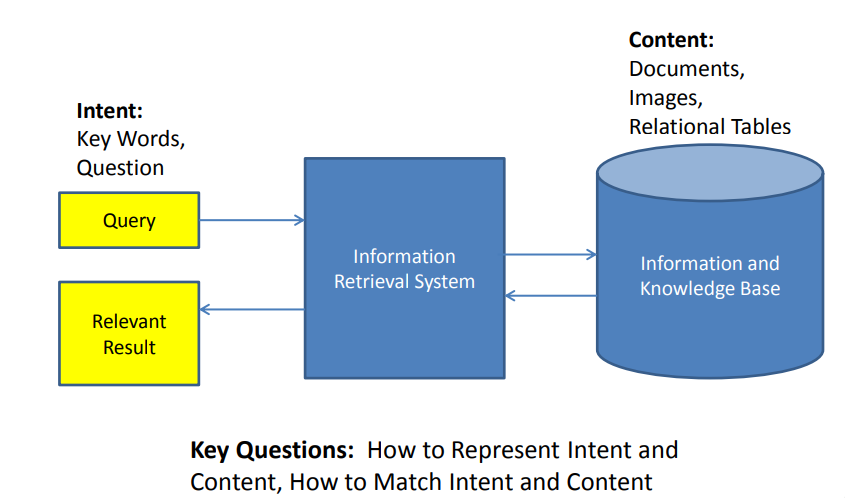
\includegraphics[width=8cm,keepaspectratio]{image/overviewIR.PNG}}
	\label{fig:docpublish}
\end{figure}


\subsection{Why Deep Learning in IR?}

First we explain why IR? When a user wants to something that he hears about but he not know what’s it actually is. Then he try to represent his information need in form of some words. And search it on some IR system such as Google. When system receive a query, it represents query and documents in same form and then try to find documents that are most relevant to that query and return that documents to user. User read these documents and finally his information need fulfilled. But the difficulty is how to represent information need and content and how to find matching scores of them. We know many ways in IR but they based on syntax. For example when a user made a query, system find that documents where these words exists and rank them according to their frequencies or some other statistical measures. But this does not mean these documents actually relevant to the user query. For this we need semantic matching between query and documents. This is the point where deep learning comes in to IR. 

Many deep learning based techniques are used in many IR areas. For example, semantic matching of query and documents is a major task of web search. Because for efficient and accurate retrieval of content semantic matching is necessary. Syntax matching not guarantee the accuracy. And also deep leaning techniques~\cite{mitra2017neural} are used to ranks documents and later on we will discuss some working related to this.  

\subsection{Hard Problems in IR Used Deep Learning Based Solutions}

But we not have all of the information in same form. We have information in many forms how to match information that not in same form. For example we have some information in the form of tables (structured data), most of the information are in unstructured form and some in multimedia form how to direct match these different forms of data. Many method and techniques available for image retrieval and question answering but their performance is not satisfactory. These problems of IR are called hard problems and deep learning is used as a tool to solve these hard problems. Because deep learning is very powerful tool, it has the capability to learn different forms of data for different problems and can represent it in some same form and because it learn some patterns from content and these learned information in same form. It improves the accuracy of many IR tasks that first looks like impossible. But now lot of work is done to introduce deep learning in different areas of IR~\cite{pang2016text}. 

\begin{figure}[h]
	\centerline{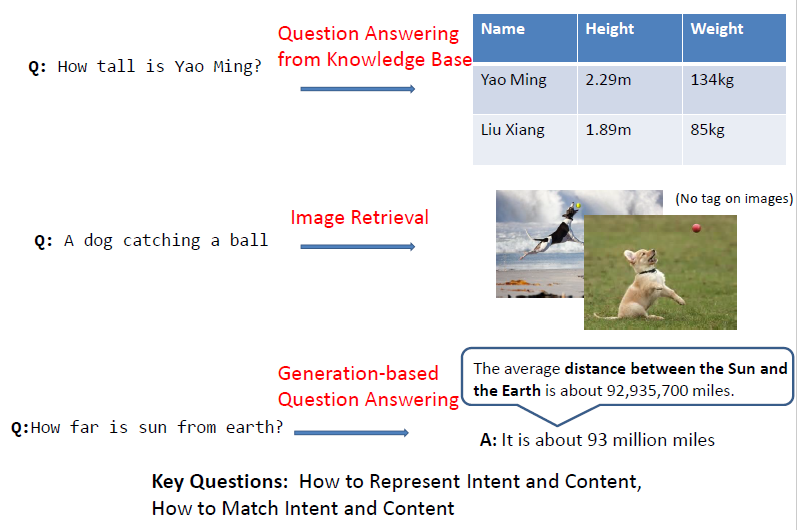
\includegraphics[width=8cm,keepaspectratio]{image/hard_problem_IR.PNG}}
	\label{fig:Hard Problems in Information Retrieval}
	\caption{Hard Problems in Information Retrieval}
\end{figure}



\section{Basics of Deep Learning} \label{sec:deeplearningoverview}

\subsection{Neural Network}
Neural network~\cite{8540494} concept comes from human brain. Its considered that our brain contain many small units that are highly interconnected to each other. These units are called perceptron. Perceptron~\cite{ramchoun2016multilayer} is a small unit that takes some number of inputs and multiply each input corresponding to its weight and sum them. After that result passed through an activation function and that output some value. Perceptron also called neuron. 


\begin{figure}[h]
	\centerline{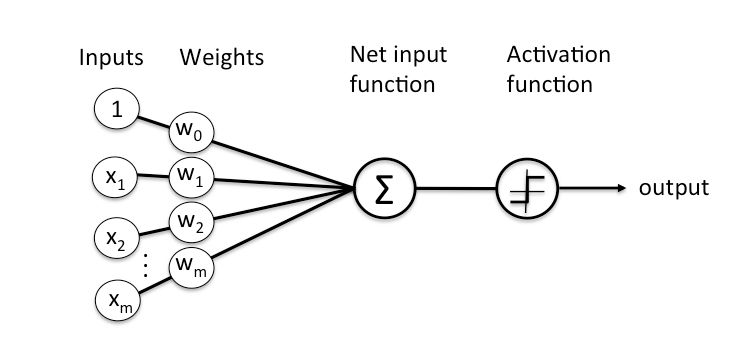
\includegraphics[width=8cm,keepaspectratio]{image/perceptron.PNG}}
	\label{fig:Percptron}
	\caption{Perceptron or Single Layer Network}
\end{figure}

Basically, a neural network consists of two or more layers. First layer called input layer and last layer called output layer and intermediate layers are hidden layers. Neurons of each layer are independent of each other but the output of neurons of previous layer becomes input for next layer neurons and same process repeated to last layer. Each circle in the figure shows a neuron. Internal working of each neuron is same as shown in Figure 3. When a neural network has 50  or more hidden layers then its comes to be known as deep learning.  

\begin{figure}[h]
	\centerline{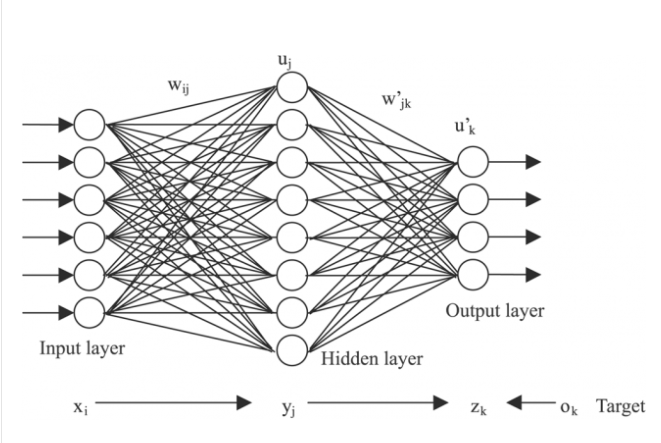
\includegraphics[width=8cm,keepaspectratio]{image/nn.PNG}}
	\label{fig:Neural Network}
	\caption{Neural Network With single Hidden layer}
\end{figure}
\subsection{Word Embedding}
Word2vec~\cite{kenter2015short} is a method whose input is a corpus of documents and its output is a set of vectors. Each vector is in numeric form. It’s a 2 layer neural network not a deep neural network. But the output generated by Word2vec is acceptable by a deep neural network. Word2Vec actually used to group similar words together without human intervention. It’s a mathematical model. Word2vec actually uses to recognize the meaning of the word with respect to its previous occurring and in which context this word occur. Word2vec detect association of one word to other (e.g. “boy” is a man). And also cluster documents of same context at one place and can classify these clusters that can help in search related tasks. Now, each word has a vector associated to it that can be used as input in deep learning neural networks and it can give back relationships between words. 
The vectors discussed above that are used as representation of word are called neural word embedding’s.  From above we can say that neural word embedding is actually a way to represent a word as number. But most important thing of this is that for training it’s not used word itself but it uses words that are closer to that word semantically and syntactically means similarity based on vector representation of word with other words. This can be done in two ways. We can learn a target word by using its context (continuous bag of words or CBOW~\cite{mitra2017neural} ) and from a word we can learn its context (skip-gram). A basic overview of these two methods in shown in Figure 3.  


\begin{figure}[h]
	\centerline{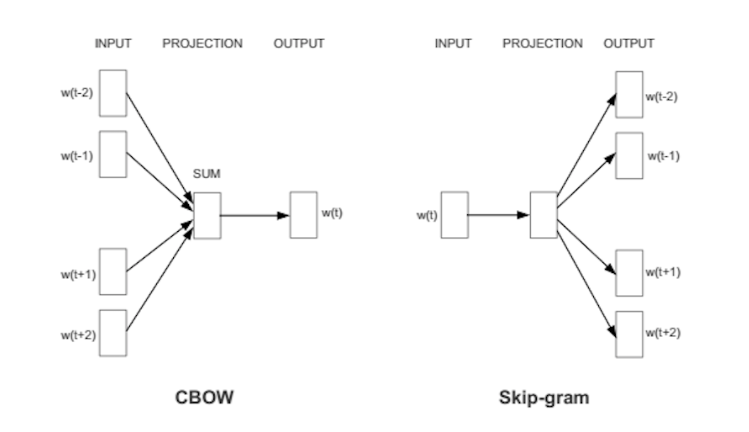
\includegraphics[width=8cm,keepaspectratio]{image/word-embeddings.PNG}}
	\label{fig:Two methods of Word Embedding}
	\caption{Two methods of Word Embedding}
\end{figure}

When the context of word is not correctly classified by the feature vector of word then the components of the feature vectors adjust themselves so that context of word correctly classified by the word. It means context of word acts as a teacher for vector of word. The basic idea is to place similar words closer to each other. 



\subsection{Recurrent Neural Network} In recurrent neural network~\cite{7804882} output of previous step becomes input of next step. In IR task most of the time we consider words independent of each other. This is the approach in which each word occurrence depends on previous some words occurrences. Its used when we have to predict the next word in the sentence. Word occurrence in a sentence depends on its previous words. Each recurrent neural network has three gates. One is to discard irrelevant information from the memory that is no further needed for next word prediction. And one gate is used to save the information after each step when this information needed for some incoming words prediction and last gate to give the prediction of current step. This is high level view of recurrent neural network it will be discussed latter in IR context in detail. 

\begin{figure}[h]
	\centerline{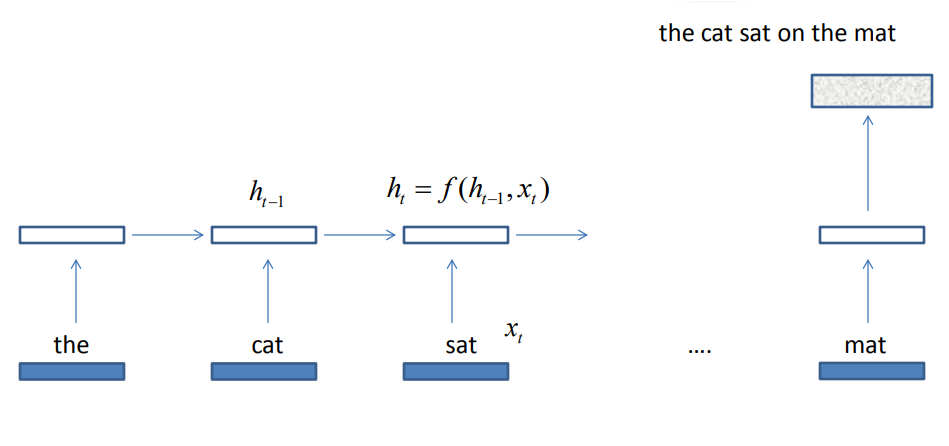
\includegraphics[width=8cm,keepaspectratio]{image/rnn.PNG}}
	\label{fig:Recurrent Neural Network}
	\caption{High Level View of Recurrent Neural Network}
\end{figure} 


\subsection{Convolutional Neural Network}

Convolutional Neural Network~\cite{7804882,shen2014latent,severyn2016modeling} is a neural network. But its hidden layers can belong to some various types that are discussed below.

\begin{itemize}
	\item {\em Fully Connected layer} A fully connected layer is a layer that takes input from all neurons of previous layer and compute its output based on all previous layer neurons.
	\item {\em Convolutional Layer} In contrast to fully connected layer, this layer takes input only from a restricted neurons of previous layer and these restricted neurons are called receptive fields of that neuron.
	\item {\em Pooling layer} This layer~\cite{shen2014latent} neurons considers that previous layer neurons are mapped in to k number of clusters and based on some criteria it chooses one neuron from each cluster and take it as input and compute output by this method. For example if we consider each neuron give some real value as output and we make 4-neurons in one cluster then it choose input from that cluster that has maximum value.  
	
	
\end{itemize}


\begin{figure}[h]
	\centerline{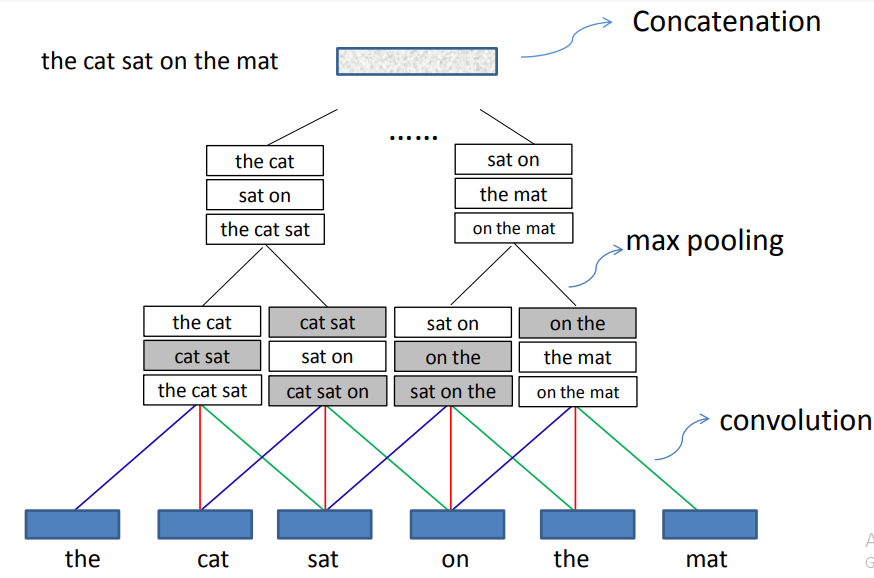
\includegraphics[width=8cm,keepaspectratio]{image/cnn.PNG}}
	\label{fig:Convolutional Neural Network}
	\caption{Convolutional Neural Network}
\end{figure} 

\section{Fundamental Problems in Deep Learning for IR}
\subsection{Learning of Distributed Representation}
In information retrieval, we deal with huge collection of documents and text and we have to search based on some query. But query is user dependent and our task to better understand the query and make relevant documents rank top on the rank list. One of the major problem is how to represent a word. In IR, we consider all distinct words as vocabulary, and represent each word in high dimensional vector that has all of its components zero instead of one component. We can extend this representation for sentence. But how it becomes a deep learning problem? We have to represent a sentence in a vector that can have many of distributed information inside it. For example information about syntax, semantic, and order and many other information. This problem can be easily handled with the help of neural networks that are basic unit of deep learning and gradient based errors are used for performance enhancement of these system.  
\subsection{Matching}
In IR, we deal with texts and matching is simply the matching of two texts or strings. In IR, two types of matching problems 1)query and document matching 2)question and answer matching. Many deep neural network based approaches for matching exists and some of them are
\begin{itemize}
	\item {\em Projection to Latent Space} Represent both query and document or question and answer in vector space with the help of some neural network~\cite{shen2014latent,severyn2016modeling,lu2013deep}. Then simply make decision based dot product of their vector representation. Neural network based three approaches are there 1) CNN~\cite{shen2014latent,severyn2016modeling} 2) DNN 3) RNN. This model is actually, the extension of basic vector space model. 
	\item {\em One Dimensional Matching} Represent both question and answer with the help of CNN and then combine both representations in to one. And apply tensor network or deep neural network on it and after that compute matching score between them~\cite{qiu2015convolutional,hu2014convolutional}. 
	\item {\em Two Dimensional Matching} Two dimensional model of question and answer passed from the Convolutional neural network and then combined representation of both question and answer is taken as input of deep neural network that give matching score as output~\cite{pang2016text,wan2016deep}.  
	\item {\em Tree Matching} Represent both question and answer in the form of tree. Then matching pattern techniques of trees are used  to compute matching representation of question and answer that is also an tree that is input of deep neural network that return matching score as output~\cite{wang2015syntax}. 
		
\end{itemize}
\subsection{Translation}
Translation is the task to transform one string in to other. In IR, translation related problems are 
\begin{itemize}
	\item Answer generation from question 
	\item Search related problem query generation
\end{itemize}

Approaches for translation problems are 

\begin{itemize}
	\item {\em Sequence to Sequence learning} Sequence to sequence learning is to represent both question and answer as sequence of fixed dimension. Question and answer can both be taken as sequences of text. But of different dimensions. This is major problem that how to represent these sequences as of fixed dimensions. Many of the methods exist for example this problem is solved with the help of neural networks.It is long short term memory(LSTM) related model that uses a hierarchical structure. This model uses some kind of encoding and decoding same as in case of RNN ~\cite{sutskever2014sequence}. 
	\item {\em RNN Encoder-Decoder} This model consists of two RNN. One is used to encode the input sequence in to fixed length vector and the other is used for decoding of intermediate representation in to the target sequence. This model tries to maximize the condition probability of generating the target sequence from the input sequence ~\cite{cho2014learning}. This model keep track of both syntax and semantic of sequence and generate intermediate representation based on both.  
	\item {\em Attention Mechanism}
\end{itemize}

\subsection{Classification}

Classification is to assign a label to a string. In IR, the tasks related to classification involves classification of query, document,question and answer in to different topics. Means classify them according to their topic or category structure. Three approaches are there to handle classification in IR. 
\begin{itemize}
	\item {\em World Level Model} It divides the input sentence into words and these words are used for further processing and called word level embedding. This model is used for classification of sentences. Inputs are word embeddings that are passed from CNN or DNN that results an representation of sentence and a softmax classifier is used to classify or compute score. 
	\item {\em Character Level Model} It divides the input sentence into sequence of characters such that each sequence consists of k consecutive characters and called character level embedding.Input is sentence and character embeddings of sentence passed from deep convolutional neural network, that gives a document representation. This representation passed through 3-layer fully connected neural network that results in document classification~\cite{zhang2015character}. 
	\item {\em Hierarchical Model} Used for document classification. Input is document that is passed from RNN and gives representation of all sentences inside documents. These representations are combined into single vector that is passed again from RNN and document representation is the result that is passed from softmax classifier and classify document title and topic~\cite{yang2016hierarchical}.  
\end{itemize} 
\subsection{Structured Prediction}
Structured prediction is the task to transform a string in to its structure. In IR, its about to recognize entities and their relationship from query, document or from question or answer.
Three approaches are there to handle Structured Prediction in IR. 
\begin{itemize}
	\item {\em CNN} 
	\item {\em Sequence-to-Sequence Learning}
	\item {Neural Network based Parsing}
\end{itemize}  

\section{Applications of Deep Learning to IR}

\subsection{Search}
Search is related to enter a query and then information system have to make search based on all terms of query and return all of the relevant documents that are available inside large collection of documents(millions or billions). Many of click through data can be used for ranking of documents and system can learn from past experience. When a user enters a query and receive results from a system, and click on some relevant results. This click can be used for future similar queries. Deep learning can be easily used to learn things from experience or something like supervised learning. An overview of search related problem is given in figure below. 
\begin{figure}[h]
	\centerline{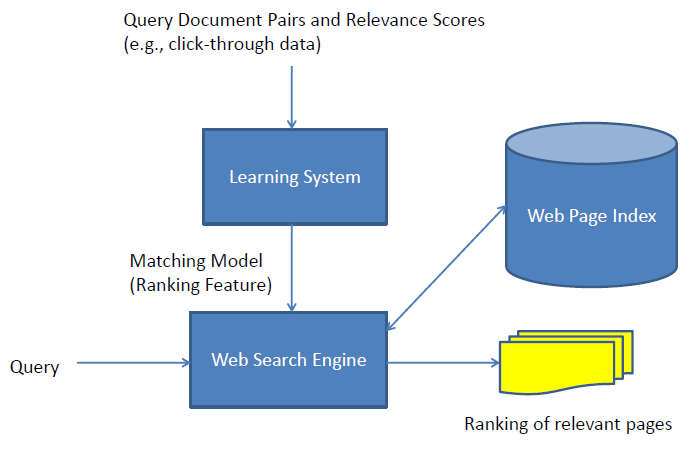
\includegraphics[width=8cm,keepaspectratio]{image/search.PNG}}
	\label{fig:Query Document Retrieval Problem}
	\caption{Query Document Retrieval Problem}
\end{figure} 
One of the model built for query document retrieval problem is Deep Structured Semantic Model(DSSM)  and complete architecture of this problem is discussed in next section. A general model of retrieving relevant documents from query is given in the figure below. This model represents both query and documents in the form of vectors that preserve some semantic of texts for matching of both query and document. Then word hashing is applied on these vectors. This is tri-letter hashing same as tri-gram letter model in which we use three letters to create representations of individual words. Then this vector resulting after word hashing is passed from some layers of neural network. After that at last layer a similarity function is used to make scoring of each document based on their degree of relevance to query. And the final score is some conditional probabilities that gives the likelihood of query generation from a given document~\cite{huang2013learning}.  
\begin{figure}[h]
	\centerline{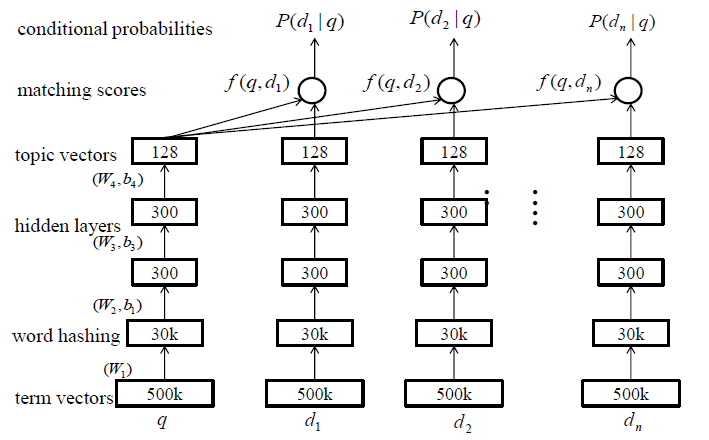
\includegraphics[width=8cm,keepaspectratio]{image/search-problem-solution-model.PNG}}
	\label{fig:General Model of Document Retrieval based on query}
	\caption{General Model of Document Retrieval based on query}
\end{figure}


Why tri-letter hashing? Direct vector representation of query and document can be used as input to neural network. The benefits of using tri-letter hashing are first it reduces the error rate as many representation of same words it can be more helpful in case of spelling mistakes. If a word contain some letter mistake inside it, then many of tri-letters sequences are same as for original word if we use directly the word itself, then it results in mismatch. But this results in collisions means, many different word can have some patterns of tri-letter hashing same, but these collisions are tolerable and not more than a specific range. 

\begin{figure}[h]
	\centerline{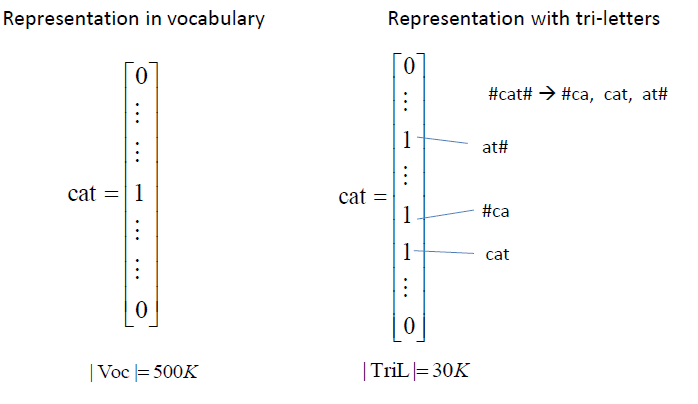
\includegraphics[width=8cm,keepaspectratio]{image/tri-letter-hashing-example.PNG}}
	\label{fig:Tri-letter Hashing Example}
	\caption{Tri-letter Hashing Example}
\end{figure}

Many of the deep learning based neural network solutions exit for matching and ranking problems. Matching and ranking models can be easily combined one after the other. But matching model must be first used and then output of this model used for ranking model as input. The working of matching model is same as Convolutional neural network that is briefly described in previous section. And ranking model working is based on deep neural network that takes feature vector learned by matching model and try to find best score for that document.  

\subsection{Question Answering (from Documents)}
\subsubsection{Retrieval-based Question Answering}

What is Retrieval-based Question Answering System? A system takes question as its input. It has facts or some knowledge base where actual question and answer pairs are saved. The main purpose of this system is to match the new question with some known question. Then the answer of this known question will be answer of new question. In this case, the question text is actually a short text and its more important to purely understand the semantics of question instead of syntax match. An example of Retrieval-based Question Answering is given in below figure. 

\begin{figure}[h]
	\centerline{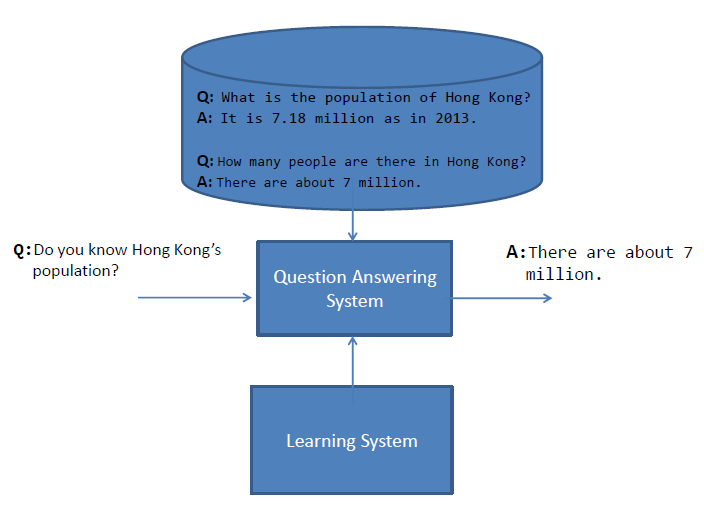
\includegraphics[width=8cm,keepaspectratio]{image/retrieval-based-QA.PNG}}
	\label{fig:Retrieval-based Question Answering}
	\caption{Retrieval-based Question Answering Example}
\end{figure}
Retrieval-based Question Answering System first try to find relevant questions and answer pairs from the given knowledge base. Then from retrieved answers it have to compute matching score for each answer and return the answer that have maximum score from all of them. A general overview of this system is shown in figure below. Deep learning based solution of this problem uses convolutional neural network for semantic matching. Two types of architectures are used. One represent both question and answer as vectors and compute matching score of them. This is known as Deep Match CNN (Architecture I). Second model uses two dimensional view for computing matching of two sentences. And this is known as Deep Match CNN (Architecture II) . This architecture is discussed in detail in next section~\cite{hu2014convolutional,ji2014information}.  
\begin{figure}[h]
	\centerline{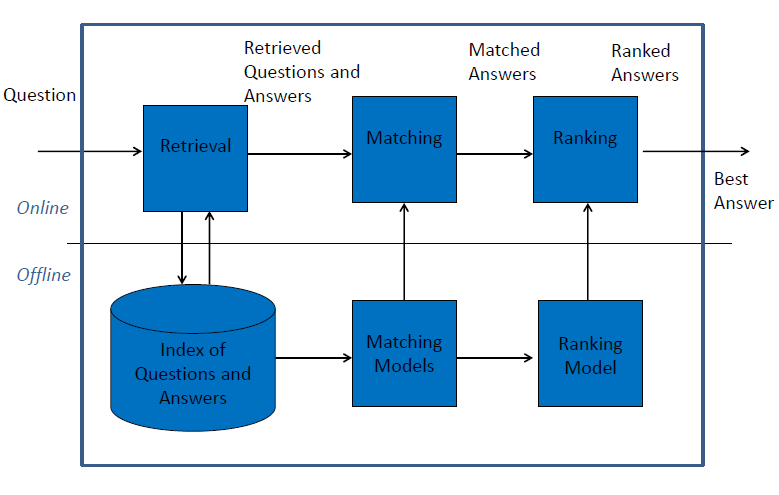
\includegraphics[width=8cm,keepaspectratio]{image/retrieval-based-QAS.PNG}}
	\label{fig:Retrieval-based Question Answering System}
	\caption{General Retrieval-based Question Answering System}
\end{figure}

\subsubsection{Generation-based Question Answering}
what is Generation-based Question Answering? Some known facts are store in knowledge base. With the help of these facts we generate an answer for a question that user enters. First the relevant facts to this question are determined. Then semantically use all relevant facts to generate an answer. An example of Generation-based Question Answering is shown in figure below. The solution to this problem in deep learning is the neural responding machine model. This machine makes use of encoder and decoder. First it encodes the input sentence into some internal representations and some preprocessing is performed on it. After that, in final step, we decode this internal representation in to answer. This machine is GRU based approach. Encoder is combination of some local and global encoders and decoder mechanism same as attention mechanism discussed in case recurrent neural network encoder and decoder ~\cite{shang2015neural}.  


\begin{figure}[h]
	\centerline{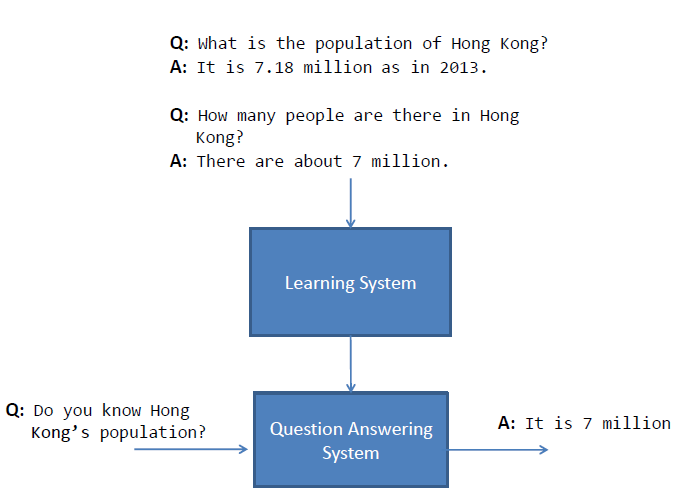
\includegraphics[width=8cm,keepaspectratio]{image/generation-based-QA.PNG}}
	\label{fig:Generation-based Question Answering}
	\caption{Generation-based Question Answering}
\end{figure}


\subsection{Question Answering from Relational Database}
 Same as retrieval based question answering except that in that instead of documents collection, we have a structured database. That store information related to some specific domain. For example, information related to employees of a specific company is in the form of tables. Each column of table belong to some specific domain. From question, we have to recognize different field values and then exact matching of values applied. This task is same of retrieval from sql database. 


\begin{figure}[h]
	\centerline{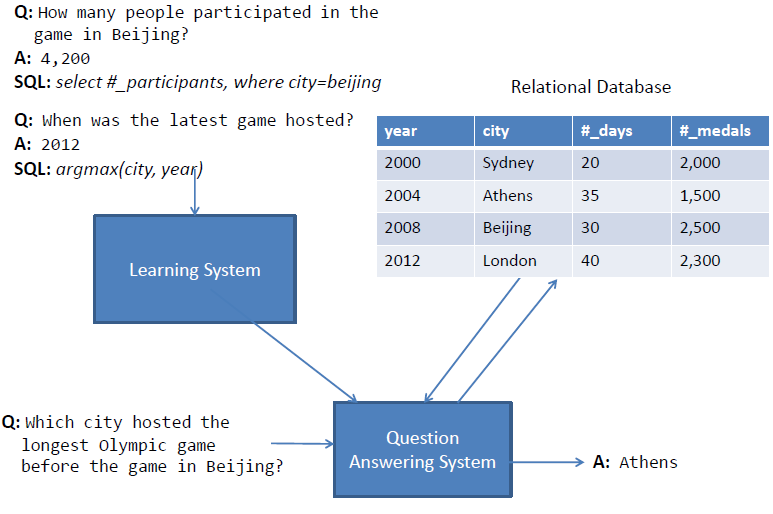
\includegraphics[width=8cm,keepaspectratio]{image/relational-QA.PNG}}
	\label{fig:Question Answering from Relational Database}
	\caption{Question Answering from Relational Database}
\end{figure}
\subsection{Question Answering from Knowledge Base}

Instead of relational tables, data is in the form of knowledge base tables. These tables also have fields like relational database~\cite{yin2015neural}. A detailed of this is discussed in next section first part. 
\subsection{Image Retrieval}

One of the major problem in IR, is how to conclude some information from an image. And how to match an image and text. This is difficult task because of image and text representations are different. The key idea of this problem is to semantically conclude some facts from an image. then these facts can be used for matching with text. Solution in deep learning for this problem is multi-model CNN. This model represent both image and text as vectors. Then similarity measure of these two vectors is not an issue. Three levels of matching are used for matching word, sentence and phrase level matching. And discussed in detail in next section~\cite{ma2015multimodal}. 

\begin{figure}[h]
	\centerline{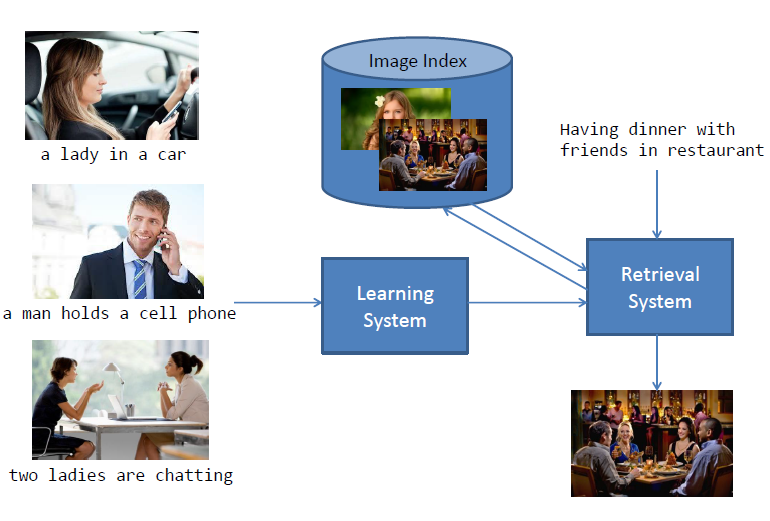
\includegraphics[width=8cm,keepaspectratio]{image/image-retrival.PNG}}
	\label{fig:Image and text matching}
	\caption{Image and text matching}
\end{figure}

\section{Architecture of Some Proposed Deep Learning based IR Model}

\subsection{Neural Enquirer Model for Question Answering based on Knowledge Base}
This model based on knowledge base table(KBT). This table contain information about some specific area and we consider it in the form of structured data because each table has specified number of fields that are fixed. For example, we consider a match tournament related KBT, this table contains fields like year country, score and some specific attributes. But the major problem is hear how to detect which value belong to which attribute. Because inside query we not specify field value, we only give some sentence that has mix up of all these fields. How to separate them. First we think how a human think. For example we have a sentence that has US inside it. Our main focus is on this word in the sentence. Neural Enquirer model thinks like humans. It takes a query and understand what its semantically mean by. And this query in the form of vector. I not discussed how to encode query semantically, i only give a high level view of this paper here. Query encoding done by a system unit that is called encoder. 
\begin{figure*}[t]
	\centerline{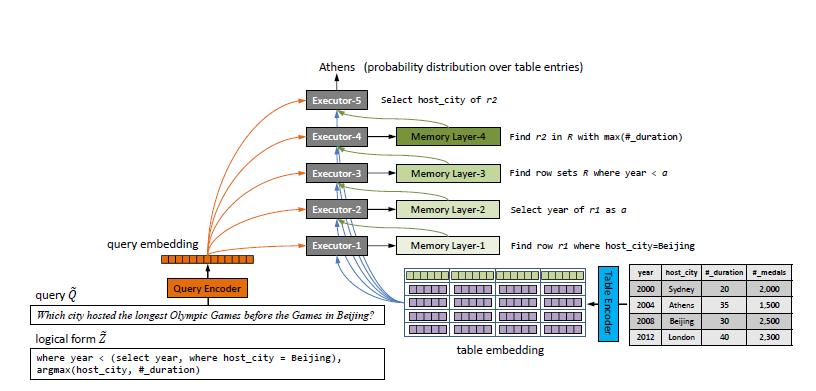
\includegraphics[width=\textwidth]{image/neuralENQUIRER.PNG}}
	\label{fig:neuralENQUIRER}
	\caption{Overview of Neural Enquirer}
\end{figure*} 
 
 Executor is another unit of Enquirer that takes query encoding and KBT and perform some computations and conclude refine question to some way and output it. Actually,  Neural Enquirer is a network network and instead of neurons we consider each layer has executor inside it and output of one executor becomes input of the next executor. The response of previous executor is temporarily stored in memory, so that next layer can use it. The final output only computed at the last layer. At the last layer KBT not used but it directly returns probability of given answer. Executor is a two step process it consists of reader and annotator. Reader reads a row of KBT according to query encoding and store and after some computation stored it in memory of that executor and after reader all of the rows relevant to that executor in memory. After that from all of the rows a generalized annotation discovered based on all of the row annotations and compute table annotation and store it in external memory and annotations performed by a unit that is called annotator. The Process of executor l is given in figure ~\ref{fig:executor}. 


\begin{figure}[h]
	\centerline{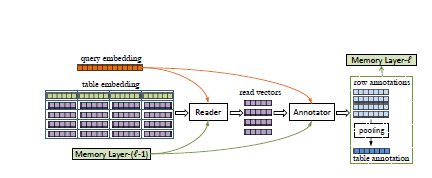
\includegraphics[width=8cm,keepaspectratio]{image/executor.PNG}}
	\caption{Executor Unit Processing Overview}
	\label{fig:executor}
\end{figure} 

Table annotation is like a pooling layer that i discussed in convolutional neural network. It summarizes all of the row annotation of a single layer in to one and make a global prediction. Row annotations of previous layer not used in next layer only the table annotation layer is used.  The out put layer of neural network not perform annotations computation it only gives probability of the final answer. For training of this model an end to end(N2N) approach of this model used that not take care of intermediary states. But input and Output states has high influence on training. A Step by Step(SbS) approach is already there that takes cares of all intermediary steps. And SbS approach is more accurate than both of N2N and OOV-N2N(out of vocabulary N2N approach). A simple version of neural enquirer is able to deal with unseen events. It divides vocabulary word in to two types. One is operation words that matters on execution of query such as before and after some year. And some words are entity words that are country names etc. This approach handle absence of operation words~\cite{yin2015neural}.  
\subsection{Learning to Rank Short Text Pairs with Convolutional Deep Neural Networks}
The Paper~\cite{severyn2015learning} formulate solution to Answer selection problem. We have a question, many candidates are  their that can be its answer, We have to select an accurate and efficient answer. Many of the ranking algorithms are there, that tackles many of features such as related to their syntax, semantic and lexicon. But these are complex and many of the computations are their to make a feature vector based on the above. When feature vector, then many of the similarity measures are that are used how much two vectors(query and document vector) are similar. In this paper, a deep learning based solution is proposed for this answer selection problem. I shortly discuss this deep learning in below paragraphs. 

The main units of this deep learning model are two sentence model that are distribution and their working is based on the convolutional neural network. This model works in two passes. In first pass, it process query and documents, make their distributional feature vectors and using some similarity measure to keep track of their semantic distribution. This is the model, that perform matching of query and documents based on their semantic and model based on deep learning neural network. 
\begin{figure*}[t]
	\centerline{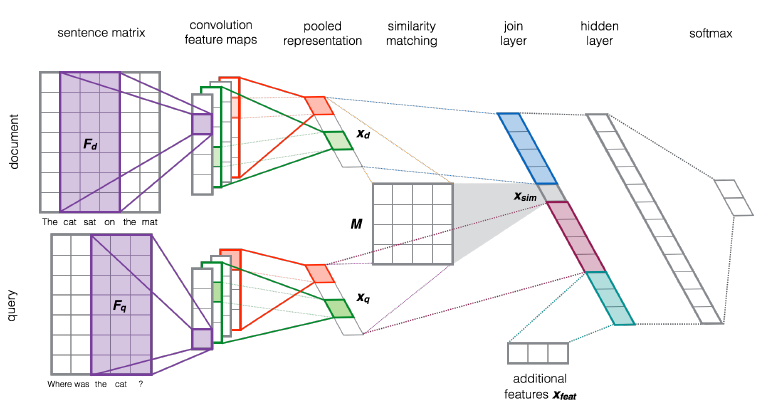
\includegraphics[width=\textwidth]{image/rerankshorttextpairs.PNG}}
	\caption{Deep Learning architecture for re-ranking short text pairs.}
	\label{fig:rerankshorttextpairs}
\end{figure*} 

The intermediate representation of feature vectors tried to take best than all previous model, so that a good semantic matcher can be built from it. This model using only a single wide layer of convolutional layer and after that a single max pooling layer.The input of this model is a raw text, whose some internal representation is created and passed through phases of this model.The high level overview of this model is shown in figure ~\ref{fig:rerankshorttextpairs}. The basic setting of convolutional neural network for this is described below.

\begin{figure}[h]
	\centerline{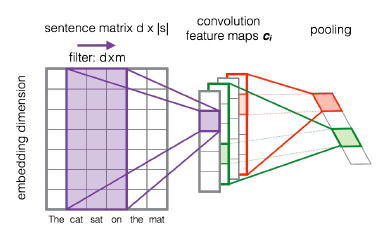
\includegraphics[width=8cm,keepaspectratio]{image/shortpair.PNG}}
	\caption{Sentence model for mapping input sentences to their intermediate feature representations}
	\label{fig:sentencemodel_shortpair}
\end{figure} 

In the above Figure ~\ref{fig:sentencemodel_shortpair}, the matrix represent sentence matrix in which each row correspond to a sentence that is a sequence of words and columns of that matrix correspond to vocabulary words. The purpose of convolutional layer is to extract the discriminative patterns of sequence of words from the input sentence. Two varieties of this layer one is wide and the other is narrow, it differently restricts the filter size that is applied on input sentence,  the wide size layer handle words at boundaries of sentence better and it assigns equal weights to all words in the sentence. while opposite in narrow range. This model use wide convolutional layer. 

To make a neural network be able to learn non linear functions, is to use non-linear functions as activation units. The non-linear activation units are tan hyperbolic function, sigmoid function and ReLU(Rectified linear unit). The activation function changed, result in different results with different convergence rate. For this model rectified linear unit activation function is used because of its advantages over other activation units. The output from convolutional layer after applying activation function becomes input of pooling layer. And pooling layer function is to a make generalize view of the representational vector. The above steps are repeated for both query and documents and after that similarity between both of vectors is determined by the following formula. 
\begin{equation}\label{key}
sim(x_{q},x_{d}) = x_{q}.M.x_{d}
\end{equation}

In above equation, M is a similarity matrix. In hidden layer that is added before the softmax layer, the interactions between internal components are modeled. The softmax layer compute probability distribution for each label. For parameter optimization of neural networks stochastic gradient descent with back propagation method is used. The deep learning method proposed in this paper not require extra parsers. And its performance is comparable with other syntactic parsers. This is the recent research in answer selection task and it improves about 3\% MAP and MRR compare to previous methods. 

 
\subsection{Convolutional Neural Tensor Network Architecture for Community-based Question Answering}

Community-based Question Answering(CQA)~\cite{qiu2015convolutional} is an online service that becomes popular in recent some years. In this system, CQA websites exists, where a user can post his question. And other users can view the questions and can answer his question. But the problem is that, users not cares, that relevant question already exist and answered by users, a user represent his question in his own words and post it. By lexical point of view, their may be large gap between this question and previous question but semantically they both same. An example of these questions is shown in figure ~\ref{fig:questionretrival}. 
\begin{figure*}[t]
	\centerline{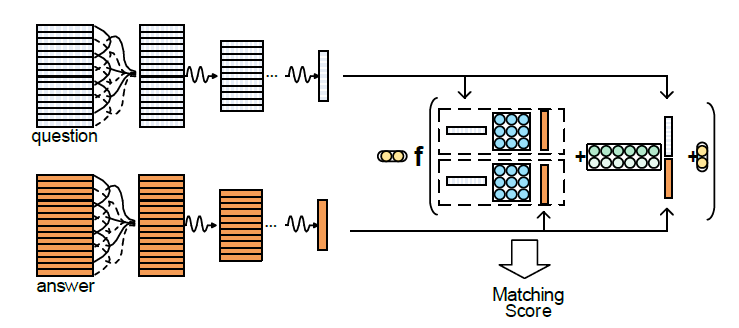
\includegraphics[width=\textwidth]{image/NTN.PNG}}
	\caption{Architecture of Neural Tensor Network.}
	\label{fig:NTN}
\end{figure*}

\begin{figure}[h]
	\centerline{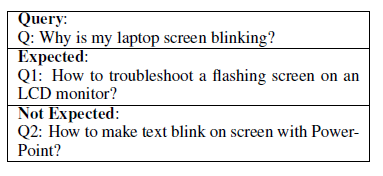
\includegraphics[width=8cm,keepaspectratio]{image/questionretrival.PNG}}
	\caption{An Example of Question Retrieval}
	\label{fig:questionretrival}
\end{figure} 

In the figure above, the query is semantically same to question 1. When user enter this as new question, then this question will point to original question and its answer. So, next time if some semantically same query comes, it point to all its possible answers. 

Convolutional neural tensor network(CNTN)~\cite{qiu2015convolutional} integrate two layers together. one is sentence modeling and the other is semantic matching. The input word tokens are converted in to vector representation by using lookup layer. Then encoding of both questions(query) and documents(answer) in to fixed length vectors using convolutional and pooling layer. After that matching scores are computed between question and answer using tensor layer. This model groups similar question and answers in semantic vector space and try to reduce the effect of lexical gap problem discussed above. 

\textbf{Neural Sentence Model} Many deep learning based methods are there that use neural network to represent or model sentences. One of them is Neural bag of words (NBOW), but major drawback of this approach is that it not consider the order of words in a sentence. This can be useful in case of general document classification but not used in short sentence matching. The other is recurrent neural network (RNN) that consider order of words but latest words in the sentence has more impact on it and sentence is biased toward last words. The other is recursive neural network, it needs some external parse tree related methods. The most important method is convolutional neural network  that uses convolutional and pooling layer to represent variable length sentences in to fixed length vectors. CNN is more important than others due to the following two reasons. 


\begin{figure}[h]
	\centerline{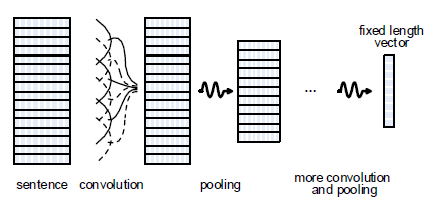
\includegraphics[width=8cm,keepaspectratio]{image/sentencemodeling.PNG}}
	\label{Sentence modelling with convolutional neural network}
	\caption{Sentence modeling with convolutional neural network}
\end{figure} 


\begin{itemize}
	\item It takes care of sequence of words in a sentence, that more important part of classification of short texts or sentences.
	\item  It uses non-linear activation function that is more powerful function to represent any kind of function. 
	
\end{itemize}

Both the question and answer are passed from the layers of Convolutional neural network. First it passed from convolutional layer and then passed through k max-pooling layer. Value of k is determined by some experiments that are performed again and again on some data and then a generalize value of is used that give better performance. After that a non-linear tan hyperbolic function is used and after that in the final layer, a fixed length vector is obtained. Means question and answer are represented in to fixed length vector using two convolutional neural network. After that, to measure similarity of question and answer both are passed from a tensor layer. Tensor is a geometric object that is used to measure similarity of two vectors and with other tensor objects. The final output of convolutional neural network is the matching score between two texts. 



\subsection{Syntax-Based Deep Matching of Short Texts}

This paper~\cite{wang2015syntax} is about to calculate the matching score between two short texts. The proposed method is considered as two components.
\begin{itemize}
	\item The first component is to represent each sentence in the form of dependency tree and discover patterns that can help to determine similar texts in the product space of dependency tree.
	\item  The second component is to determine the matching score between two short texts using deep neural network. 
	
\end{itemize} 
\begin{figure*}[t]
	\centerline{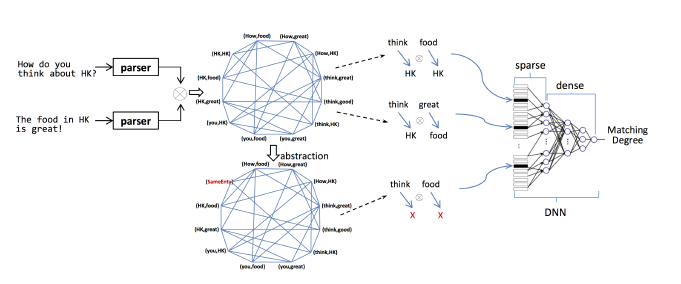
\includegraphics[width=\textwidth]{image/syntax-based-dl.PNG}}
	\caption{Architecture of Syntax based deep learning}
	\label{fig:Architecture of Syntax based deep learning}
	\end{figure*}
Each sentence is represented by a dependency tree. This tree actually store long term and short term relations of all words in a sentence. An example of a Chinese tweet and its corresponding dependency tree is given in figure ~\ref{fig:dt}. The bold face words inside a sentence need not to be directly connected to each other. 
\begin{figure}[h]
	\centerline{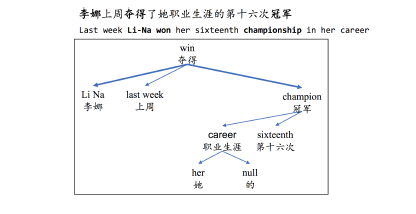
\includegraphics[width=8cm,keepaspectratio]{image/dt.PNG}}
	\caption{An Example of dependency tree. The tweet is in Chinese (literal English translation).}
	\label{fig:dt}
\end{figure} 

When we make dependency trees of short texts, then the next step is to combine them. The direct dot product method is used to combine them. Means dot product of question and answer dependency tree is measured. And an example of two dependency trees with their dot product is shown in figure ~\ref{fig:product-dt}. The dot product of two simple dependency trees is in the form of highly interconnected graph. Two types of abstractions are performed on this graph. 
\begin{figure}[h]
	\centerline{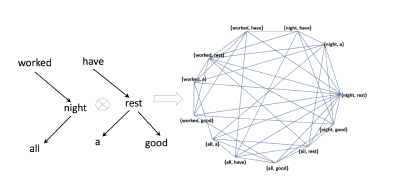
\includegraphics[width=8cm,keepaspectratio]{image/product-dt.PNG}}
	\caption{The direct product of two dependency trees}
	\label{fig:product-dt}
\end{figure} 

\begin{itemize}
	\item{\em Same Entity} This abstraction is applied on vertices's of the graph. The idea is here to represent same entity in a graph by a general vertex.  
	\item{\em Similar Words} This type of abstraction is also applied on  of the graph. It's based on clustering method that is discussed already in basic of deep learning section. 
\end{itemize}
Both of these abstractions, to make a generalized view of the patterns of dot product of dependency trees of each sentence. Abstraction gives the model, that gives more general view and its results more better than method applied without abstraction.

\subsection{A Deep Relevance Matching Model for Ad-hoc Retrieval}


Ad hoc retrieval task~\cite{guo2016deep} ia actually formulate as matching of two texts according to their relevance. The model in this proposed paper is called deep relevance matching model(DRMM). Three main factors of relevance matching model are
\begin{itemize}
	\item Histogram Matching
	\item  Feed forward based neural matching network
	\item  Term gating network
\end{itemize}


\textbf{Types of Deep Matching Models}

Two most important types of deep matching models are 
\begin{itemize}
	\item{\em Representation-focused Model} This model focus on good representation of individual texts and then deep neural network based model is used to compute matching score of them.   
	\item{\em Interaction-Focused Model} This model try to find local interactions between two short texts. And then try to find the hierarchical interaction between texts using deep learning based neural network. These two types are shown in figure ~\ref{fig:Types of deep Macting Models}.
\end{itemize}

\begin{figure*}[t]
	\centerline{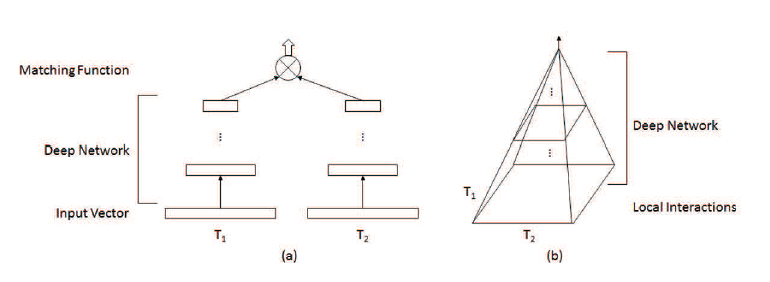
\includegraphics[width=\textwidth]{image/types-matching-models.PNG}}
	\caption{Types of deep Matching Models: a)Representation-focused Model b)Relevance Matching Models}
	\label{fig:Types of deep Macting Models}
\end{figure*}  

Most of the matching models designed are semantic matching models that try to match two texts semantically. But, this approach based on relevance matching. And this model is based on interaction-focused model. DRMM try to find all possible local interactions between each pair of query and document and try to make histogram mapping from it. Then a feed forward neural network model is used to build actual hierarchical relations and a matching score is determined. At the last stage, each query document pair score is used to generate aggregated score overall using term gating network. 

\begin{figure}[h]
	\centerline{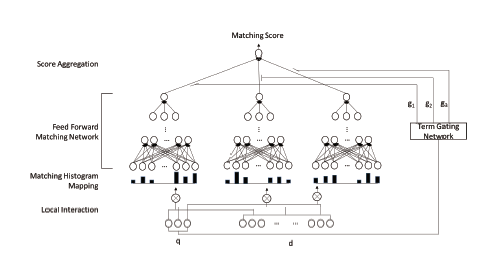
\includegraphics[width=8cm,keepaspectratio]{image/deep-relevance-matching-model.PNG}}
	\caption{Architecture of the Deep Relevance Matching Model.}
	\label{fig:Architecture of the Deep Relevance Matching Model}
\end{figure} 

 Local interactions between each query and document term is built. But these interactions are of variable length due to different lengths of query and documents. Previous methods used matching matrix to represent these interactions. And matrix preserve position related information that is not important in relevance matching problem. So, instead of matching matrix, histogram based representation is used and value in each histogram is the number of total interactions in each bin. To make value in limited range, these values in histogram are normalized. After that, log of count value is computed to make range shorter. An overview of complete architecture of this model is shown in figure ~\ref{fig:Architecture of the Deep Relevance Matching Model}
\subsection{Hierarchical Recurrent Encoder with Latent Topic Clustering}


Previous Recurrent Dual Encoder Model uses recurrent neural network to represent both query and documents. This model not used this because of this fails in case of long sequences of texts. But, some extensions already exist that tries to handle long sequence of sentences. This not handle this problem in generalize way. The solution of this is Hierarchical Recurrent Dual Encoder. 
\begin{figure}[h]
	\centerline{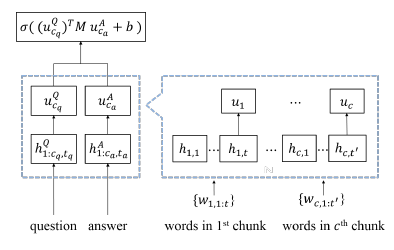
\includegraphics[width=8cm,keepaspectratio]{image/HRDE.PNG}}
	\caption{Hierarchical Recurrent Dual Encoder Model}
	\label{HRDE model}
\end{figure}
This method divides the long sequences of texts into chunks of short sentence, short paragraphs and chunks of some words. Word level RNN, making encoding of word sequences inside a single chunk. And this process is repeated for each chunk. We have output of Word level RNN equal to total number of chunks made of long sequence of texts. Chunk level RNN combines all of the word level RNN outputs to make a single representation of each text. This chunk level RNN keep sequential order of each word level RNN. The second part of this model is the latest topic clustering(LTC)~\cite{yoon2017learning}, that tries to cluster topics in general view of the document topic and also topic related to query. After that, topic of both query and documents are matched. That, makes an enough improvement in achieving better results. 

\begin{figure}[h]
	\centerline{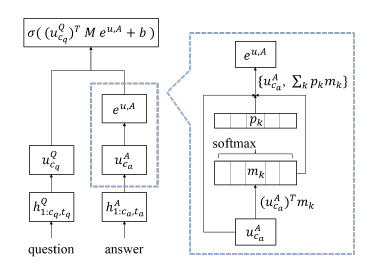
\includegraphics[width=8cm,keepaspectratio]{image/HRDE-LTC.PNG}}
	\caption{Diagram of the Hierarchical Recurrent Dual Encoder with Latent Topic Clustering (HRDE-LTC)}
	\label{Diagram of the HRDE-LTC}
\end{figure}

\subsection{Dual Attention Networks for Multimodal Reasoning and Matching}
This model is the solution to image and text problems. For example we have lot of images and we want to infer the information from these image. or we want to make decisions on the basis of images. How we can do that? For this the only thing, is to determine what's happening inside an image semantically. Then we have text representation of images, now we can compute its similarity with text and we return images as answer to texts. This model uses the intensity difference between pixels to detect things and to detect what is done inside images. An overview of Dual attention network problem~\cite{nam2016dual} is shown in figure below.

Both of the image and text have their own representations called image representation and text representation respectively. Two of the attention mechanisms are there:
\begin{itemize}
	\item{\em Visual attention} Visual attention is about to represent different parts inside input image. This process is repeated for k steps and each result will be result in improvement. So, what value of k used it's also depend.    
	\item{\em textual attention} This phase takes input sentence as input and create its representation. Same k representations of textual attentions are created and used inside model. 
\end{itemize}

This model uses two different models for two different type of problem. Both of the models use k visual and textual attention steps to compute the final answer. But, the computations for both of these models are different and we not discussed these computations here. These two models are

\begin{itemize}
	\item rDAN for Visual Question Answering   
	\item mDAN for Image Text Matching
\end{itemize}

\begin{figure}[h]
	\centerline{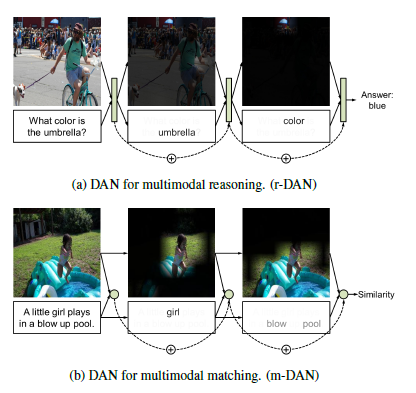
\includegraphics[width=8cm,keepaspectratio]{image/DAN.PNG}}
	\caption{Overview of Dual Attention Networks (DANs)
		for multimodal reasoning and matching.}
	\label{DAN}
\end{figure}
\section{Discussion}
From all of the above discussion and reading, we make some observations about models that are better than others. CNN and RNN both are used for matching of two text or for ranking of documents~\cite{ma2015multimodal}. CNN model gives more accurate results than RNN. and 2-dimensional CNN model gives more accurate results than 1-dimensional model~\cite{hu2014convolutional}. But performance of tree pattern matching problems depends on the training data available. There accuracy will be more than CNN and RNN and it performs more better than these two models, but training data must be enough to recognize correct feature vectors and patterns. If training data contains errors, it also effect of accuracy of model~\cite{wang2015syntax}. RNN is more suitable for answer generation problems from fact of KB and translation related problem. And more dimensional track more information than lower dimensions. So, high dimensional models gives more accurate results than lower. And performance of RNN can be improved by using attention mechanisms. This improves both accuracy and efficiency of it ~\cite{bahdanau2014neural}.  

CNN model mostly used for classification problems and its accuracy is more than RNN model. This model can be used for sentence and document classifications and many of the papers are there that discussed about each of these classifications ~\cite{kim2014convolutional,lai2015recurrent}. And input of these classification uses different levels of embeddings. These embeddings can be of word, character and of sentence levels. And commonly a neural network that has two layers inside it, used for document level classification ~\cite{yang2016hierarchical}. In most of information retrieval tasks, bag of words model performs more well than model that make computations based on syntax based models. Bag of words is actually consider document as sequence of words and characters and making shingles of them that can be on the base of characters and words. And then computing similarity between them. These are probability based models and sometimes called naive Bayes model ~\cite{iyyer2015deep}. In structured prediction type problems, deep learning  is not widely used. Some of the deep models are there that gives performance approximately equal or slightly greater than other state-of-the-art problems. This is the area where deep learning need much more of research for improvement of results ~\cite{andor2016globally}. 

The effect of deep learning in all fundamental problems areas of information retrieval is given in figure ~\ref{fig:dl-result}. This figure shows the importance of deep learning in all problem areas of IR where deep learning can be applied to solve problems. In each area performance of deep learning based algorithms is comparable with basic solutions available. And problems related to matching, translation and classification areas, improves their results by usage of deep learning based techniques. And already discussed, structured prediction needs some future work for further improvements. And the benefit of using deep learning is that it not requires much of the domain knowledge to solve each kind of problem. It means they can be easily understandable~\cite{huang2013learning}. 
\begin{figure}[h]
	\centerline{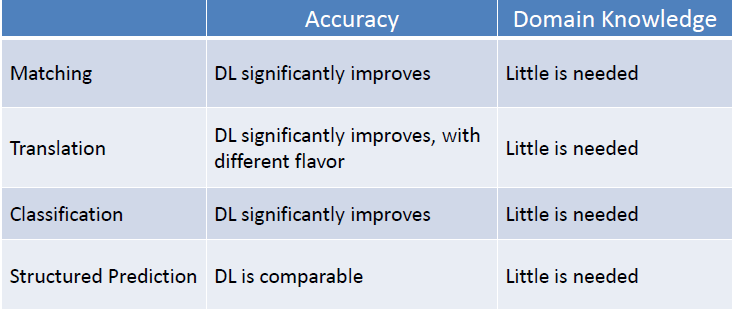
\includegraphics[width=8cm,keepaspectratio]{image/dl-IR-areas.PNG}}
	\caption{Comparison of Deep Learning(DL) with State-of-the-Art for Fundamental Problems}
	\label{fig:dl-result}
\end{figure}

Deep Structured Semantic Model (DSSM) that is used for document retrieval. This model is trained by using approximately the 100,000,000 of query and document pairs. This date is generated by using click data that is used for indirect relevance feed back. This data is generated based on this and when user make a query and system return some documents and user click on some of them. This information is used to mark that this document is relevant to that query. And for many of the queries this information is saved. And for testing approximately 15,000 queries are used and each of the query have same number of relevant documents to avoid any of the inconvenience due to some query have more relevant documents. The NDCG (Normalized Discounted Cumulative Gain)  is computed for DSSM and for other state-of-the-art models available. The results shown that DSSM performs well than others models. And results of this experiment is shown in figure ~\ref{fig:DSSM-result}.
\begin{figure}[h]
	\centerline{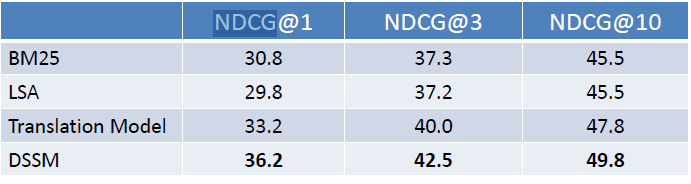
\includegraphics[width=8cm,keepaspectratio]{image/DSSM-result.PNG}}
	\caption{Comparison of DSSM with State-of-the-Art Models}
	\label{fig:DSSM-result}
\end{figure}

CNN is used for ranking and matching of documents. And its performance is tested by using TREC collection of question and answer pairs. For training 53,000 question and answer pairs from TREC collection are used and for testing 13,000 pairs are used from same collection and performance of CNN is compared with other state-of-the-art problems. For performance measure MAP and MRR are used and CNN results shows that it improves performance in terms of accuracy~\cite{severyn2015learning}. 

\begin{figure}[h]
	\centerline{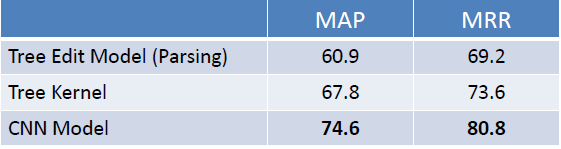
\includegraphics[width=8cm,keepaspectratio]{image/CNN-result.PNG}}
	\caption{Comparison of CNN with State-of-the-Art Models}
	\label{fig:CNN-result}
\end{figure}

Deep Match Models for Retrieval-based Question Answering are also compared with other state-of-the-art models. For training of models Weibo data (Chinese) collection is used with approximately 4.4 million of data. And about 70\% of the accuracy was found for this system ~\cite{hu2014convolutional,ji2014information} and result are shown in figure ~\ref{fig:DMMresult}.
\begin{figure}[h]
	\centerline{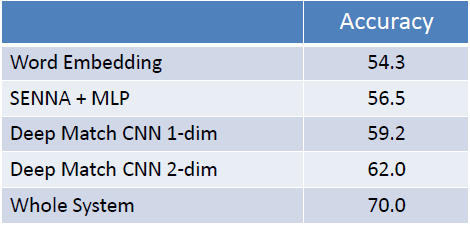
\includegraphics[width=8cm,keepaspectratio]{image/DMM-result.PNG}}
	\caption{Retrieval-based Question Answering Models Accuracy}
	\label{fig:DMMresult}
\end{figure}

Generation based Question Answering experiment is done on Chinese Weibo pairs of question and answer and this model is 76\% accurate ~\cite{shang2015neural}. An example message and response for this model is shown in figure ~\ref{fig:g-qa}. 
\begin{figure}[h]
	\centerline{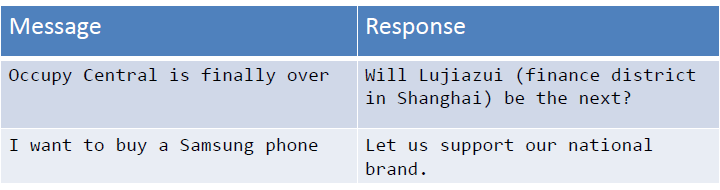
\includegraphics[width=8cm,keepaspectratio]{image/g-qa.PNG}}
	\caption{Generation based Question Answering Result}
	\label{fig:g-qa}
\end{figure}

Question-Answering from Knowledge Base gives approximately 52\% of accuracy. This experiment is done by using a Chinese collection of question answer pairs and this data is noisy means many of the errors regarding answer generation in training data. Due to which performance of this model is not very high. This performance can be very high if training data is free of noise and all of the facts from which we generate our answer need to be correct. An example of answer generation with some given question is shown in figure~\ref{fig:a-kb}. Approximately 720,000 question answer pairs are used for training and KB consists of 1.1 million of rows~\cite{yin2015neural}.   
\begin{figure}[h]
	\centerline{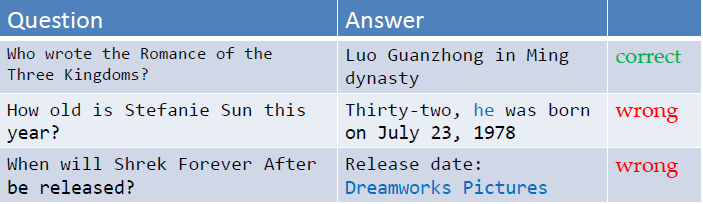
\includegraphics[width=8cm,keepaspectratio]{image/a-kb.PNG}}
	\caption{Question Answering from Knowledge Graph Result}
	\label{fig:a-kb}
\end{figure}

Multi-Model convolutional network that is used for text and image matching task. Its performance is compared with other state-of-the-art model by using recall @ K measure and results shown that this outperforms than all other models~\cite{ma2015multimodal}. The table is shown in figure ~\ref{fig:M-CNN-result}. This model was trained by using 30,000 data of Flickr collection. 
\begin{figure}[h]
	\centerline{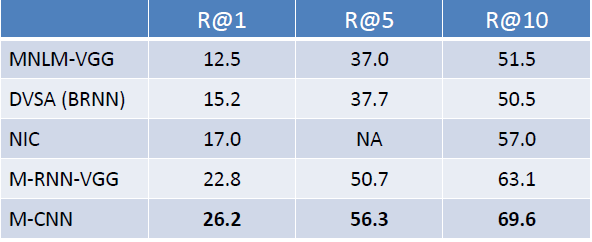
\includegraphics[width=8cm,keepaspectratio]{image/M-CNN-result.PNG}}
	\caption{M-CNN comparison with other state-of-the-art models}
	\label{fig:M-CNN-result}
\end{figure}
\section{Future Work}
Symbolic processing has its own benefits. Its easier to control and direct effective. And neural processing(deep learning) is robust to noisy data, flexible(adaptable for each type of environment or problem). And neural processing is data driven based model. But the major problem in IR is how to combine both of the symbolic processing and neural processing? This is major challenge in IR that needs future research on it\cite{li2016deep}. 

Structured Prediction related deep learning solutions not showing extra-ordinary improvement in results. This area need more research for accuracy and efficiency improvement.  
\section{Conclusion}
Deep learning is one of the most popular machine learning tool that is approximately used in all areas of study and its results are more accurate than all models. In this paper, we identify some fundamental problem areas of IR, where deep learning is successfully applied and good performance is achieved than other state-of-the-art models. In matching, translation, and classification related IR problems, deep learning significantly improve performance. But in structured prediction area, performance is comparable with other state-of-art models. This area need research for improvement. CNN model is better than RNN models. And it's used for document and sentence classification problems. Accuracy of RNN can be further improved by using attention mechanisms. And high dimensional models give more accurate results than low dimensional problems. Performance of these models can be increased sufficiently if our training data is free of noise and some more accurate models are developed. So, each area of IR, need some more research according to deep learning point of view. Because deep learning is so powerful tool that it can represent any complex pattern. 

%\section*{Acknowledgement}
%The project is funded in part by the National Institutes of Health, under Grant No. 5R01CA136535.


%%%%%%%%%%%%%%%%%%%%%%%%%%%%%%%%%%%%%%%%%%%%%%%%%%%%%%%%%%%%%%%%%%%%%%%%%%%%%%%%%%%%%

\bibliography{ref}
\bibliographystyle{unsrt}

%\bibliographystyle{alpha}

\end{document}
